% !TeX program = xelatex
\documentclass{article}
\usepackage{kotex}
\usepackage[a4paper,left=3cm, right=3cm, top=2cm, bottom=2cm]{geometry}
\usepackage{amsmath}
\usepackage{graphicx}
\usepackage{caption}
\usepackage{setspace}
\usepackage{xcolor}
\usepackage{titlesec}
\usepackage{amssymb}
\usepackage{tcolorbox}
\usepackage{wrapfig}
\usepackage{amsthm}
\usepackage{multirow} 
\usepackage{array}
\usepackage{tcolorbox}
\usepackage{pgfplots}
\pgfplotsset{compat=1.18} % For proofs

\graphicspath{{graph/}}
\title{7.4 특성방정식}
\date{}
\author{}
\setstretch{1.3}

% \subsection* 형식 지정 (번호 없음)
\titleformat{name=\section, numberless}
  {\normalfont\large\bfseries\color{blue}}
  {}
  {0pt}
  {}
\geometry{a4paper, margin=1in}

% 증명 환경 스타일
\newtheoremstyle{mystyle}% name
  {}% Space above
  {}% Space below
  {\itshape}% Body font
  {}% Indent amount
  {\bfseries}% Theorem head font
  {.}% Punctuation after theorem head
  {.5em}% Space after theorem head
  {}% Theorem head spec (can be left empty, meaning `normal')
\theoremstyle{mystyle}

\begin{document}
\maketitle

\begin{tcolorbox}[colback=blue!5, colframe=blue!60!black, title=7.4 특성방정식 -- 한눈에 보기, boxrule=0.5mm, arc=3mm]
이차곡면의 대칭축(주축) 방향을 구하는 3차방정식이 \textbf{특성방정식}이다.
\[
t^3-It^2+Jt-D=0,\qquad I=a+b+c,\quad J=ab+bc+ca-f^2-g^2-h^2,\quad D=\begin{vmatrix}a&h&g\\h&b&f\\g&f&c\end{vmatrix}
\]
세 근 \(t_1,t_2,t_3\)에 대응하는 세 방향은 \textbf{서로 직교}하며, 각 방향에 수직인 평면이 \textbf{주경면}이다.
\end{tcolorbox}

\begin{tcolorbox}[
    colback=teal!4,
    colframe=teal!65!black,
    title=정의 \& 핵심 규칙,
    fonttitle=\bfseries,
    boxrule=0.5mm,
    arc=3mm
    ]
    \textbf{\textcolor{teal!65!black}{정의.}}\quad
    방향코사인이 \(\lambda,\mu,\nu\)인 현들의 중점을 모으면 다음 평면을 얻는다.
    \[
    (a\lambda+h\mu+g\nu)x+(h\lambda+b\mu+f\nu)y+(g\lambda+f\mu+c\nu)z+l\lambda+m\mu+n\nu=0 \tag{①}
    \]
    이를 방향 \(\lambda,\mu,\nu\)에 \textbf{공액인 경면}이라 하고, 경면에 의해 이등분되는 현을 \textbf{종선}이라 한다. (유심이차곡면이면 경면은 항상 중심을 지난다.)

    \noindent\textcolor{teal!50!black}{\rule{\linewidth}{0.4pt}}

    \textbf{\textcolor{teal!65!black}{핵심 규칙.}}\quad
    종선과 경면이 \textbf{직교}(즉 곡면이 그 평면에 대해 대칭)하는 방향 \(\lambda,\mu,\nu\)를 구하면, 그 방향은 반드시 아래 특성방정식의 근이어야 한다. 근에 수직인 경면을 특별히 \textbf{주경면}이라 한다.
\end{tcolorbox}

\textbf{유도.} 방향코사인 \(\lambda,\mu,\nu\)인 직선과 경면 ①이 직교할 조건은
\[
\frac{a\lambda+h\mu+g\nu}{\lambda}=\frac{h\lambda+b\mu+f\nu}{\mu}=\frac{g\lambda+f\mu+c\nu}{\nu}
\]
이므로 이 공통값을 \(t\)로 놓으면
\[
(a-t)\lambda+h\mu+g\nu=0,\qquad h\lambda+(b-t)\mu+f\nu=0,\qquad g\lambda+f\mu+(c-t)\nu=0 \tag{②}
\]
을 얻는다. 이 식이 \(\lambda,\mu,\nu\) 모두 0은 아닌 해를 가지려면
\[
\begin{vmatrix} a-t & h & g\\ h & b-t & f\\ g & f & c-t \end{vmatrix}=0 \tag{③}
\]
이어야 하고, 이를 \textbf{특성방정식}이라 한다. 역으로 ③의 근 \(t\)를 ②에 대입해 \(\lambda:\mu:\nu\)를 구하고 \(\lambda^2+\mu^2+\nu^2=1\)로 정규화한 뒤 ①에 대입하면
\[
t(\lambda x+\mu y+\nu z)+l\lambda+m\mu+n\nu=0
\]
인 \textbf{주경면}의 방정식을 얻는다.

특성방정식 ③을 전개하면
\[
t^3-It^2+Jt-D=0 \tag{④}
\]
\[
I=a+b+c,\qquad J=ab+bc+ca-f^2-g^2-h^2,\qquad D=\begin{vmatrix} a&h&g\\ h&b&f\\ g&f&c \end{vmatrix}
\]

\begin{tcolorbox}[
    colback=red!4,
    colframe=red!60!black,
    title=정리 1,
    fonttitle=\bfseries,
    boxrule=0.5mm,
    arc=3mm
    ]
    특성방정식 ③의 서로 다른 두 근 \(t_1,t_2\)에 대응하는 두 방향은 서로 \textbf{직교}한다.
\end{tcolorbox}

\begin{proof}
\(t_1,t_2\)에 대응하는 방향코사인을 각각 \((\lambda_1,\mu_1,\nu_1),(\lambda_2,\mu_2,\nu_2)\)라 하면 각각 ②를 만족한다. \(t_1\)에 대한 식들에 순서대로 \(\lambda_2,\mu_2,\nu_2\)를 곱해 더하면
\[
a\lambda_1\lambda_2+b\mu_1\mu_2+c\nu_1\nu_2+h(\lambda_1\mu_2+\lambda_2\mu_1)+f(\mu_1\nu_2+\mu_2\nu_1)+g(\nu_1\lambda_2+\nu_2\lambda_1)-t_1(\lambda_1\lambda_2+\mu_1\mu_2+\nu_1\nu_2)=0
\]
같은 방법으로 \(t_2\)에 대해서도 좌변이 같은 식을 얻고, 두 식을 빼면
\[
(t_1-t_2)(\lambda_1\lambda_2+\mu_1\mu_2+\nu_1\nu_2)=0
\]
\(t_1\ne t_2\)이므로 \(\lambda_1\lambda_2+\mu_1\mu_2+\nu_1\nu_2=0\), 즉 두 방향은 직교한다.
\end{proof}

% ============ 이미지 삽입 위치: 정리1 직후 -- 서로 직교하는 세 주축(고유방향) ============
% 기울어진 이차곡면(좌표축과 나란하지 않음) 위에 서로 수직인 세 방향 t1,t2,t3를 표시.
% "특성방정식의 세 근에 대응하는 방향이 서로 직교한다"는 정리1을 시각적으로 보여줌.
\begin{figure}[h]
\centering
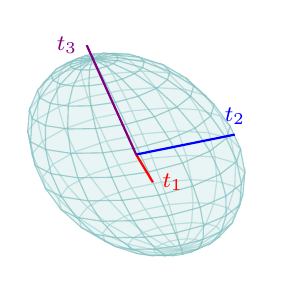
\begin{tikzpicture}
\begin{axis}[hide axis, view={115}{20}, width=6cm, height=6cm]
\addplot3[
    surf, shader=faceted, faceted color=teal!55, fill=teal!12, opacity=0.45,
    domain=0:180, domain y=0:360, samples=14, samples y=18, z buffer=sort,
]
(
  {2*sin(x)*cos(y)*cos(25) - 1.1*sin(x)*sin(y)*sin(25)},
  {(2*sin(x)*cos(y)*sin(25) + 1.1*sin(x)*sin(y)*cos(25))*cos(20) - 1.4*cos(x)*sin(20)},
  {(2*sin(x)*cos(y)*sin(25) + 1.1*sin(x)*sin(y)*cos(25))*sin(20) + 1.4*cos(x)*cos(20)}
);
\addplot3[thick, red]    coordinates {(0,0,0) (1.722,0.755,0.275)};
\addplot3[thick, blue]   coordinates {(0,0,0) (-0.465,0.937,0.341)};
\addplot3[thick, violet] coordinates {(0,0,0) (0,-0.547,1.504)};
\node at (axis cs:1.722,0.755,0.275) [red, anchor=west] {\footnotesize $t_1$};
\node at (axis cs:-0.465,0.937,0.341)[blue, anchor=south]{\footnotesize $t_2$};
\node at (axis cs:0,-0.547,1.504)[violet, anchor=east]{\footnotesize $t_3$};
\end{axis}
\end{tikzpicture}
\caption{좌표축과 나란하지 않은 이차곡면과 그 주축 방향 $t_1,t_2,t_3$ -- 세 방향은 서로 직교한다}
\end{figure}

\begin{tcolorbox}[
    colback=red!4,
    colframe=red!60!black,
    title=정리 2,
    fonttitle=\bfseries,
    boxrule=0.5mm,
    arc=3mm
    ]
    특성방정식 ③의 세 근이 \textbf{모두 0이 되는 경우는 없다}.
\end{tcolorbox}

\begin{proof}
세 근이 모두 0이면 ④, ⑤에서 \(I=J=D=0\)이어야 한다. 그런데
\[
I^2-2J=a^2+b^2+c^2+2(h^2+f^2+g^2)
\]
이므로 \(I=J=0\)이면 이 식이 \(0\)이 되어 \(a=b=c=h=f=g=0\)이어야 한다. 그러나 주어진 방정식은 이차방정식이므로 이는 불가능하다. 따라서 특성방정식의 세 근이 모두 0이 되는 경우는 없다.
\end{proof}

\subsection*{EXAMPLE 1}
이차곡면 \(3x^2+y^2+3z^2-2yz-2zx-2xy+4x+14y+4z-23=0\)의 주경면을 구하여라.\\
\textbf{SOLUTION:} 특성방정식은
\[
\begin{vmatrix} 3-t & -1 & -1\\ -1 & 1-t & -1\\ -1 & -1 & 3-t \end{vmatrix}=0
\quad\Longrightarrow\quad
t^3-7t^2+12t=0
\]
이므로 이를 풀면 \(t=4,\ 3,\ 0\)이다.

\(t=4\)일 때: \(-\lambda-\mu-\nu=0,\ -\lambda-3\mu-\nu=0,\ -\lambda-\mu-\nu=0\)과 \(\lambda^2+\mu^2+\nu^2=1\)을 이용하여 풀면
\[
\lambda=\frac{1}{\sqrt2},\quad \mu=0,\quad \nu=-\frac{1}{\sqrt2}
\]
따라서 주경면의 방정식은 \(x-z=0\).

\(t=3\)일 때: 같은 방법으로 풀면 \(\lambda=-\dfrac{1}{\sqrt3},\ \mu=\dfrac{1}{\sqrt3},\ \nu=-\dfrac{1}{\sqrt3}\)이고, 주경면의 방정식은 \(x-y-z-1=0\).

\(t=0\)일 때는 \(D=0\)에 대응하는 근이므로 주경면의 방정식이 \textbf{존재하지 않는다}.

\section*{연습문제 7.4}
\begin{enumerate}
    \item 다음 이차곡면의 주경면의 방정식을 구하여라.
    \begin{enumerate}
        \item[(1)] \(x^2-y^2+2z^2-2yz-2zx-2xy+2x+6y+2z-3=0\)
        \item[(2)] \(2x^2+y^2+z^2-2zx-2xy+6x-6z+10=0\)
    \end{enumerate}
\end{enumerate}
\end{document}